%% bare_conf.tex
%% V1.4a
%% 2014/09/17
%% by Michael Shell
%% See:
%% http://www.michaelshell.org/
%% for current contact information.
%%
%% This is a skeleton file demonstrating the use of IEEEtran.cls
%% (requires IEEEtran.cls version 1.8a or later) with an IEEE
%% conference paper.
%%
%% Support sites:
%% http://www.michaelshell.org/tex/ieeetran/
%% http://www.ctan.org/tex-archive/macros/latex/contrib/IEEEtran/
%% and
%% http://www.ieee.org/

%%*************************************************************************
%% Legal Notice:
%% This code is offered as-is without any warranty either expressed or
%% implied; without even the implied warranty of MERCHANTABILITY or
%% FITNESS FOR A PARTICULAR PURPOSE! 
%% User assumes all risk.
%% In no event shall IEEE or any contributor to this code be liable for
%% any damages or losses, including, but not limited to, incidental,
%% consequential, or any other damages, resulting from the use or misuse
%% of any information contained here.
%%
%% All comments are the opinions of their respective authors and are not
%% necessarily endorsed by the IEEE.
%%
%% This work is distributed under the LaTeX Project Public License (LPPL)
%% ( http://www.latex-project.org/ ) version 1.3, and may be freely used,
%% distributed and modified. A copy of the LPPL, version 1.3, is included
%% in the base LaTeX documentation of all distributions of LaTeX released
%% 2003/12/01 or later.
%% Retain all contribution notices and credits.
%% ** Modified files should be clearly indicated as such, including  **
%% ** renaming them and changing author support contact information. **
%%
%% File list of work: IEEEtran.cls, IEEEtran_HOWTO.pdf, bare_adv.tex,
%%                    bare_conf.tex, bare_jrnl.tex, bare_conf_compsoc.tex,
%%                    bare_jrnl_compsoc.tex, bare_jrnl_transmag.tex
%%*************************************************************************


% *** Authors should verify (and, if needed, correct) their LaTeX system  ***
% *** with the testflow diagnostic prior to trusting their LaTeX platform ***
% *** with production work. IEEE's font choices and paper sizes can       ***
% *** trigger bugs that do not appear when using other class files.       ***                          ***
% The testflow support page is at:
% http://www.michaelshell.org/tex/testflow/



\documentclass[conference]{IEEEtran}
% Some Computer Society conferences also require the compsoc mode option,
% but others use the standard conference format.
%
% If IEEEtran.cls has not been installed into the LaTeX system files,
% manually specify the path to it like:
% \documentclass[conference]{../sty/IEEEtran}





% Some very useful LaTeX packages include:
% (uncomment the ones you want to load)


% *** MISC UTILITY PACKAGES ***
%
%\usepackage{ifpdf}
% Heiko Oberdiek's ifpdf.sty is very useful if you need conditional
% compilation based on whether the output is pdf or dvi.
% usage:
% \ifpdf
%   % pdf code
% \else
%   % dvi code
% \fi
% The latest version of ifpdf.sty can be obtained from:
% http://www.ctan.org/tex-archive/macros/latex/contrib/oberdiek/
% Also, note that IEEEtran.cls V1.7 and later provides a builtin
% \ifCLASSINFOpdf conditional that works the same way.
% When switching from latex to pdflatex and vice-versa, the compiler may
% have to be run twice to clear warning/error messages.






% *** CITATION PACKAGES ***
%
%\usepackage{cite}
% cite.sty was written by Donald Arseneau
% V1.6 and later of IEEEtran pre-defines the format of the cite.sty package
% \cite{} output to follow that of IEEE. Loading the cite package will
% result in citation numbers being automatically sorted and properly
% "compressed/ranged". e.g., [1], [9], [2], [7], [5], [6] without using
% cite.sty will become [1], [2], [5]--[7], [9] using cite.sty. cite.sty's
% \cite will automatically add leading space, if needed. Use cite.sty's
% noadjust option (cite.sty V3.8 and later) if you want to turn this off
% such as if a citation ever needs to be enclosed in parenthesis.
% cite.sty is already installed on most LaTeX systems. Be sure and use
% version 5.0 (2009-03-20) and later if using hyperref.sty.
% The latest version can be obtained at:
% http://www.ctan.org/tex-archive/macros/latex/contrib/cite/
% The documentation is contained in the cite.sty file itself.






% *** GRAPHICS RELATED PACKAGES ***
%
\ifCLASSINFOpdf
   \usepackage[pdftex]{graphicx}
  % declare the path(s) where your graphic files are
   \graphicspath{{../pdf/}{../jpeg/}{/figures}}
  % and their extensions so you won't have to specify these with
  % every instance of \includegraphics
   \DeclareGraphicsExtensions{.pdf,.jpeg,.png}
\else
  % or other class option (dvipsone, dvipdf, if not using dvips). graphicx
  % will default to the driver specified in the system graphics.cfg if no
  % driver is specified.
   \usepackage[dvips]{graphicx}
  % declare the path(s) where your graphic files are
  % \graphicspath{{../eps/}}
  % and their extensions so you won't have to specify these with
  % every instance of \includegraphics
  % \DeclareGraphicsExtensions{.eps}
\fi
% graphicx was written by David Carlisle and Sebastian Rahtz. It is
% required if you want graphics, photos, etc. graphicx.sty is already
% installed on most LaTeX systems. The latest version and documentation
% can be obtained at: 
% http://www.ctan.org/tex-archive/macros/latex/required/graphics/
% Another good source of documentation is "Using Imported Graphics in
% LaTeX2e" by Keith Reckdahl which can be found at:
% http://www.ctan.org/tex-archive/info/epslatex/
%
% latex, and pdflatex in dvi mode, support graphics in encapsulated
% postscript (.eps) format. pdflatex in pdf mode supports graphics
% in .pdf, .jpeg, .png and .mps (metapost) formats. Users should ensure
% that all non-photo figures use a vector format (.eps, .pdf, .mps) and
% not a bitmapped formats (.jpeg, .png). IEEE frowns on bitmapped formats
% which can result in "jaggedy"/blurry rendering of lines and letters as
% well as large increases in file sizes.
%
% You can find documentation about the pdfTeX application at:
% http://www.tug.org/applications/pdftex





% *** MATH PACKAGES ***
%
%\usepackage[cmex10]{amsmath}
% A popular package from the American Mathematical Society that provides
% many useful and powerful commands for dealing with mathematics. If using
% it, be sure to load this package with the cmex10 option to ensure that
% only type 1 fonts will utilized at all point sizes. Without this option,
% it is possible that some math symbols, particularly those within
% footnotes, will be rendered in bitmap form which will result in a
% document that can not be IEEE Xplore compliant!
%
% Also, note that the amsmath package sets \interdisplaylinepenalty to 10000
% thus preventing page breaks from occurring within multiline equations. Use:
%\interdisplaylinepenalty=2500
% after loading amsmath to restore such page breaks as IEEEtran.cls normally
% does. amsmath.sty is already installed on most LaTeX systems. The latest
% version and documentation can be obtained at:
% http://www.ctan.org/tex-archive/macros/latex/required/amslatex/math/





% *** SPECIALIZED LIST PACKAGES ***
%
%\usepackage{algorithmic}
% algorithmic.sty was written by Peter Williams and Rogerio Brito.
% This package provides an algorithmic environment fo describing algorithms.
% You can use the algorithmic environment in-text or within a figure
% environment to provide for a floating algorithm. Do NOT use the algorithm
% floating environment provided by algorithm.sty (by the same authors) or
% algorithm2e.sty (by Christophe Fiorio) as IEEE does not use dedicated
% algorithm float types and packages that provide these will not provide
% correct IEEE style captions. The latest version and documentation of
% algorithmic.sty can be obtained at:
% http://www.ctan.org/tex-archive/macros/latex/contrib/algorithms/
% There is also a support site at:
% http://algorithms.berlios.de/index.html
% Also of interest may be the (relatively newer and more customizable)
% algorithmicx.sty package by Szasz Janos:
% http://www.ctan.org/tex-archive/macros/latex/contrib/algorithmicx/




% *** ALIGNMENT PACKAGES ***
%
%\usepackage{array}
% Frank Mittelbach's and David Carlisle's array.sty patches and improves
% the standard LaTeX2e array and tabular environments to provide better
% appearance and additional user controls. As the default LaTeX2e table
% generation code is lacking to the point of almost being broken with
% respect to the quality of the end results, all users are strongly
% advised to use an enhanced (at the very least that provided by array.sty)
% set of table tools. array.sty is already installed on most systems. The
% latest version and documentation can be obtained at:
% http://www.ctan.org/tex-archive/macros/latex/required/tools/


% IEEEtran contains the IEEEeqnarray family of commands that can be used to
% generate multiline equations as well as matrices, tables, etc., of high
% quality.




% *** SUBFIGURE PACKAGES ***
%\ifCLASSOPTIONcompsoc
%  \usepackage[caption=false,font=normalsize,labelfont=sf,textfont=sf]{subfig}
%\else
%  \usepackage[caption=false,font=footnotesize]{subfig}
%\fi
% subfig.sty, written by Steven Douglas Cochran, is the modern replacement
% for subfigure.sty, the latter of which is no longer maintained and is
% incompatible with some LaTeX packages including fixltx2e. However,
% subfig.sty requires and automatically loads Axel Sommerfeldt's caption.sty
% which will override IEEEtran.cls' handling of captions and this will result
% in non-IEEE style figure/table captions. To prevent this problem, be sure
% and invoke subfig.sty's "caption=false" package option (available since
% subfig.sty version 1.3, 2005/06/28) as this is will preserve IEEEtran.cls
% handling of captions.
% Note that the Computer Society format requires a larger sans serif font
% than the serif footnote size font used in traditional IEEE formatting
% and thus the need to invoke different subfig.sty package options depending
% on whether compsoc mode has been enabled.
%
% The latest version and documentation of subfig.sty can be obtained at:
% http://www.ctan.org/tex-archive/macros/latex/contrib/subfig/




% *** FLOAT PACKAGES ***
%
%\usepackage{fixltx2e}
% fixltx2e, the successor to the earlier fix2col.sty, was written by
% Frank Mittelbach and David Carlisle. This package corrects a few problems
% in the LaTeX2e kernel, the most notable of which is that in current
% LaTeX2e releases, the ordering of single and double column floats is not
% guaranteed to be preserved. Thus, an unpatched LaTeX2e can allow a
% single column figure to be placed prior to an earlier double column
% figure. The latest version and documentation can be found at:
% http://www.ctan.org/tex-archive/macros/latex/base/


%\usepackage{stfloats}
% stfloats.sty was written by Sigitas Tolusis. This package gives LaTeX2e
% the ability to do double column floats at the bottom of the page as well
% as the top. (e.g., "\begin{figure*}[!b]" is not normally possible in
% LaTeX2e). It also provides a command:
%\fnbelowfloat
% to enable the placement of footnotes below bottom floats (the standard
% LaTeX2e kernel puts them above bottom floats). This is an invasive package
% which rewrites many portions of the LaTeX2e float routines. It may not work
% with other packages that modify the LaTeX2e float routines. The latest
% version and documentation can be obtained at:
% http://www.ctan.org/tex-archive/macros/latex/contrib/sttools/
% Do not use the stfloats baselinefloat ability as IEEE does not allow
% \baselineskip to stretch. Authors submitting work to the IEEE should note
% that IEEE rarely uses double column equations and that authors should try
% to avoid such use. Do not be tempted to use the cuted.sty or midfloat.sty
% packages (also by Sigitas Tolusis) as IEEE does not format its papers in
% such ways.
% Do not attempt to use stfloats with fixltx2e as they are incompatible.
% Instead, use Morten Hogholm'a dblfloatfix which combines the features
% of both fixltx2e and stfloats:
%
% \usepackage{dblfloatfix}
% The latest version can be found at:
% http://www.ctan.org/tex-archive/macros/latex/contrib/dblfloatfix/




% *** PDF, URL AND HYPERLINK PACKAGES ***
%
%\usepackage{url}
% url.sty was written by Donald Arseneau. It provides better support for
% handling and breaking URLs. url.sty is already installed on most LaTeX
% systems. The latest version and documentation can be obtained at:
% http://www.ctan.org/tex-archive/macros/latex/contrib/url/
% Basically, \url{my_url_here}.




% *** Do not adjust lengths that control margins, column widths, etc. ***
% *** Do not use packages that alter fonts (such as pslatex).         ***
% There should be no need to do such things with IEEEtran.cls V1.6 and later.
% (Unless specifically asked to do so by the journal or conference you plan
% to submit to, of course. )

\usepackage[utf8]{inputenc}
% correct bad hyphenation here
\hyphenation{op-tical net-works semi-conduc-tor}


\begin{document}
%
% paper title
% Titles are generally capitalized except for words such as a, an, and, as,
% at, but, by, for, in, nor, of, on, or, the, to and up, which are usually
% not capitalized unless they are the first or last word of the title.
% Linebreaks \\ can be used within to get better formatting as desired.
% Do not put math or special symbols in the title.
\title{Dynamic Allocation of Serverless Functions\\ in IoT Environments}


% author names and affiliations
% use a multiple column layout for up to three different
% affiliations
\author{
\IEEEauthorblockN{Duarte Pinto}
\IEEEauthorblockA{
DEI - Faculty of Engineering,\\ University of Porto\\ Porto, Portugal}
\and
\IEEEauthorblockN{João Pedro Dias}
\IEEEauthorblockA{INESC TEC and \\
DEI - Faculty of Engineering,\\ University of Porto\\ Porto, Portugal}
\and
\IEEEauthorblockN{Hugo Sereno Ferreira}
\IEEEauthorblockA{INESC TEC and \\
DEI - Faculty of Engineering,\\ University of Porto\\ Porto, Portugal}}

% conference papers do not typically use \thanks and this command
% is locked out in conference mode. If really needed, such as for
% the acknowledgment of grants, issue a \IEEEoverridecommandlockouts
% after \documentclass

% for over three affiliations, or if they all won't fit within the width
% of the page, use this alternative format:
% 
%\author{\IEEEauthorblockN{Michael Shell\IEEEauthorrefmark{1},
%Homer Simpson\IEEEauthorrefmark{2},
%James Kirk\IEEEauthorrefmark{3}, 
%Montgomery Scott\IEEEauthorrefmark{3} and
%Eldon Tyrell\IEEEauthorrefmark{4}}
%\IEEEauthorblockA{\IEEEauthorrefmark{1}School of Electrical and Computer Engineering\\
%Georgia Institute of Technology,
%Atlanta, Georgia 30332--0250\\ Email: see http://www.michaelshell.org/contact.html}
%\IEEEauthorblockA{\IEEEauthorrefmark{2}Twentieth Century Fox, Springfield, USA\\
%Email: homer@thesimpsons.com}
%\IEEEauthorblockA{\IEEEauthorrefmark{3}Starfleet Academy, San Francisco, California 96678-2391\\
%Telephone: (800) 555--1212, Fax: (888) 555--1212}
%\IEEEauthorblockA{\IEEEauthorrefmark{4}Tyrell Inc., 123 Replicant Street, Los Angeles, California 90210--4321}}




% use for special paper notices
%\IEEEspecialpapernotice{(Invited Paper)}




% make the title area
\maketitle

% As a general rule, do not put math, special symbols or citations
% in the abstract
\begin{abstract}
The IoT area has grown significantly in the last few years and is expected to
reach a gigantic amount of 50 billion devices by 2020\nocite{kn:Cisco01}. Parallel
to IoT, serverless architectures, specifically highlighting \textit{FaaS}, are
also an increasing trend in the field of software engineering. Combining IoT with
a serverless architectural design can be effective when trying to make use of the
local processing power that exist in a local network of IoT devices and creating a
fog layer that leverages compotational capabilities that are closer to the
end-user. The proposed solution, which is placed between the device and the
serverless function, when a device requests for the execution of a serverless
function, will decide based on previous metrics of execution if the serverless
function should be executed locally, in the fog layer of a local network of IoT
devices, or if it should be executed remotely, in one of the many cloud servers.

%The solution makes this decision with the aim of improving response times, by
%taking advantage of the joint processing power of the local network of IoT devices
%when it is more beneficial and suitable to do so.
\end{abstract}

% no keywords




% For peer review papers, you can put extra information on the cover
% page as needed:
% \ifCLASSOPTIONpeerreview
% \begin{center} \bfseries EDICS Category: 3-BBND \end{center}
% \fi
%
% For peerreview papers, this IEEEtran command inserts a page break and
% creates the second title. It will be ignored for other modes.
\IEEEpeerreviewmaketitle



\section{Introduction}
Continuing the current trend, mobile data usage is expected to keep increasing
exponentially, part of it thanks to mobile video streaming and
IoT. The estimation is that the number of data that was generated
by mobile devices during the year of 2017 exceeded the $\displaystyle 6 * 10^9$ Gb
per month. Together with the traffic generated by laptops and peer-to-peer
communications, overall traffic demand might reach $\displaystyle 11 * 10^9$ Gb per
month\cite{kn:Dehos2014} \cite{kn:Baresi2017}. To compute such a big amount of
data, cloud computing would appear to be the obvious solution but there are cases
where the latency that comes with transmitting data back and forth might be
undesired. In certain situations it is also not feasible to expect a constant and
reliable internet connection to an always on server, either because it might not
be economically wise or because it might not be infrastructurally possible. In
order to solve the need for low latency, as well as to improve fault tolerance, by
not relying on an always on centralized server, serverless architectures and fog
computing aim to reduce the dependency on the cloud by making more use of the
local resources of a device and improving communication between local devices,
only leaving the data intensive tasks to the cloud\cite{kn:Baresi2017}. With the
increasing trend in serverless solutions, such as AWS Lambda, it is opportunistic
to implement this concepts in IoT.

Although IoT has been around for a few years already, the same cannot be said
about services that provide cloud solutions and cloud infrastructure for rent. 
Likewise, when Serverless and Fog Computing solutions first appeared their
usefulness and benefits for the IoT ecosystem was obvious and developers began to
mix them together in order to get the most out of these new trend.

Despite its success and the promising future for the mix of this concepts, the
area is still fairly new and few solutions can take advantage of the processing
power in the cloud and in the local network of IoT devices in an efficient way
without compromising speed. It is already possible to have a network of IoT
devices working together to execute a series of serverless functions, but not all
serverless functions are suitable to run on low-end devices. To choose where each
serverless functions should be executed (locally or in the cloud) is a manual task
and the end result is that developers choose to have all serverless functions
running in the cloud as it is easier to manage and less risky. Nonetheless, there
is a lot of potiential processing power dormant in each local network that could
be used to improve response times, improve fault-tolerance,  and to slash costs of
hosting cloud processing infrastructure. 

\section{Background}

\section{State of the Art}

\section{Problem Statement}

As stated before in previous sections, not only is expected for the number of IoT
devices to grow imensely, both commercially and industrially, but there are
already many solutions that allow for serverless functions to be executed
remotely. Due to the nature of serverless functions, some of them could perfectly
be executed locally, using the joint processing power of the multiple IoT devices.
The hardship comes with using this power efficiently, having multiple serverless
functions, and knowing where to execute each one, locally or remotely. It is not
feasible for each developer to manually analyze performance across the different
runtime environments and make a decision where the function should be executed.
This is impending the adoption of these concepts in IoT, despite the interest and
potential that exists in this evergrowing area. Not only there is a lack of
systems making use of serverless on-premises, the majority of the developers in
IoT opt for using the cloud for each and every need, disregarding the power that
exists locally.

Like what was presented above, there is a lack of practical know-how knowledge
available despite there being lots of incentives for it. There are lots of things,
but it is not easy to start developing a serverless IoT solution.

Given this, the aim of this project is to create an architecture for serverless IoT
platform and to build a proof of concept using existing open-source tools when
possible and avoiding proprietary solutions. The platform should:
\begin{itemize}
    \item Have a serverless cloud solution capable of answering HTTP requests from
        the \textit{things}.
    \item Make use of the local processing power of the multiple IoT devices to
        create a serverless virtual processing unit on the Fog Layer to answer
        local requests.
    \item Have multiple IoT devices with different functions capable of
        interacting with both the Cloud and Fog layer to execute different
        functions. 
\end{itemize}

\section{Proposed Solution}

This project tries to fix the problem stated in Chapter \ref{chap:thesis_state} by
introducing a proxy between the entity requesting the function execution and the
serverless function. This proxy will analyze each function's past history, by
looking at the time taken in past requests and make the decision of which runtime
environment \footnote{Runtime environment is the system where the serverless
function will be executed, i.e., local network or one of the servers available in
the cloud} should the request be forwarded to, see Figure
\ref{fig:request_func_high_level_diagram}. The proxy should be able to decide
between the local network of devices and one of the many available servers.

\begin{figure}[ht]
  \centering
  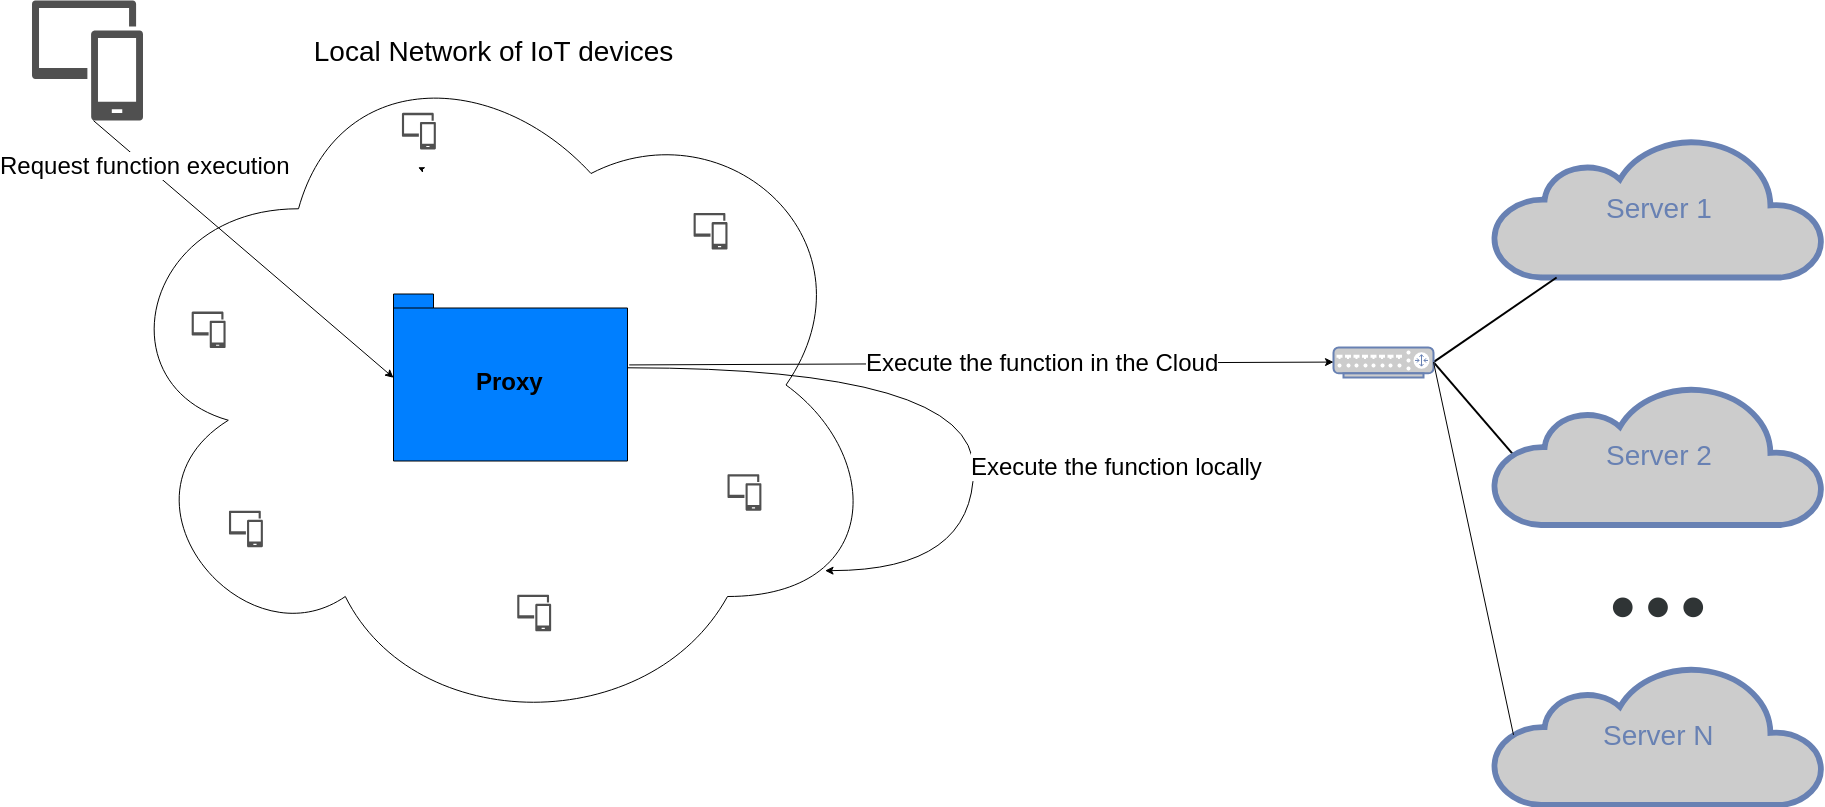
\includegraphics[width=0.5\textwidth]{diss-high-level-diagram}
  \caption{High level overview of project's architechture}
  \label{fig:request_func_high_level_diagram}
\end{figure}

In order to improve fault-tolerance, in case of no Internet connection or if
one the servers is not available, if the request to the server fails, the proxy
should fallback to the local network. This way, even if the request to execute the
function is forwarded to the server and fails, the function will still be executed
locally.

The proxy is situated inside the local network of IoT devices and will forward the
request for a specific function to a gateway which forwards the function execution to
one of the IoT devices capable of executing the function. The load management,
containerization, replication, and clustering of the serverless functions is not
handled by the proxy, but it still has to be aware of the serverless functions
installed in the local network or any of the other runtime environments.

\subsection{Expected results and flow: Use cases}
\label{overview:usecases}
The following examples explain the expected results and decision-making of the
proposed solution. The decisions taken by the proxy are based only on previous
metrics of the time taken for the runtime environment to execute the function
(including network latency).

\subsubsection{Forward function execution to the cloud} \label{usecases:forward_cloud}

The use case in Figure \ref{fig:succ-cloud-deploy} examplifies a situation where
the requested serverless function is hardware intensive, therefore taking a lot of
time to execute locally. Due to the high processing power of the cloud servers, it
is beneficial to forward the execution request to one of the cloud servers, even
when considering the connection latency. From the multiple available servers, it
will opt for the one that is physically nearest (lower latency).

\begin{figure}[ht]
  \begin{center}
    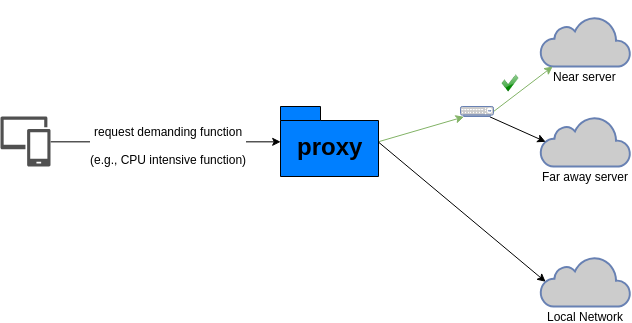
\includegraphics[width=0.5\textwidth]{diss-succ-cloud-deploy.png}
    \caption{Request for the execution of a demanding function to be executed. The
    proxy will forward the request to the cloud because due to the high processing
    power of the cloud server, the function will be executed more quickly. The nearest
    server was choosen because of latency.}
    \label{fig:succ-cloud-deploy}
  \end{center}
\end{figure}

\subsubsection{Forward function execution to the local network}
\label{usecases:forward_local}

Contrary to the previous case, the Figure \ref{fig:succ-local-deploy} portays a
scenario where the requested serverless function is very light, being more
beneficial to execute the function locally and avoid network latency. Despite the
difference in power between the two environments, the previous metrics show that
the local environment is capable of satisfying the request more quickly.

\begin{figure}[ht]
  \begin{center}
    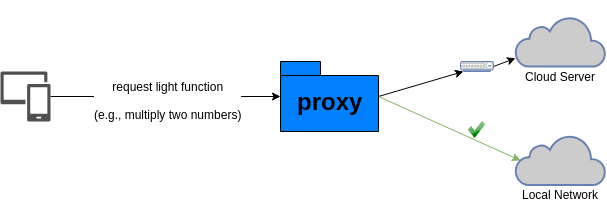
\includegraphics[width=0.5\textwidth]{diss-succ-local-deploy.png}
    \caption{Request for the execution of a simple, light function to be executed. The
    proxy will forward the request to be run locally, as there is no benefit in
    executing the function on the cloud.}
    \label{fig:succ-local-deploy}
  \end{center}
\end{figure}

\subsubsection{Fallback to the local network}
\label{usecases:fallback}

The Figure \ref{fig:fallback-local} depicts a scenario where the proxy first tries
to forward the request to one of the cloud servers (because it is more beneficial)
but fails in doing so. The proxy then decides to forward the request to the local
network, successfully completing the request. There are certain situations where
it is more favorable for the function to be executed on the cloud but it could
still be executed locally. Because it is not possible to always guarantee a
working connection, in these cases, if the connection fails the proxy will
fallback to execute function locally, assuring fail redundancy and the reliability
of the system.

\begin{figure}[ht]
  \begin{center}
    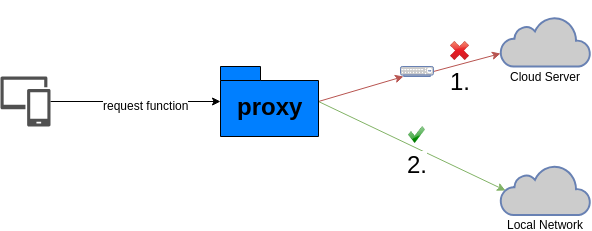
\includegraphics[width=0.5\textwidth]{diss-fallback-local.png}
    \caption{The request for the function execution to be in the cloud could not
    be satified (e.g., no internet connection). The proxy will then forward the
request for it to be executed in the local network.}
    \label{fig:fallback-local}
  \end{center}
\end{figure}

\subsubsection{Manual forward. Bypass the weighting process}
\label{usecases:manual_forward}

It should also be possible for the developer to bypass the weighting process (the
evaluation of the different runtime environments) and manually choose where to forward the
request. This option should be possible either in the setup process of the
function or as an argument of the request for the function execution. 

%\subsubsection*{Overall sequence} 
%In a very summarized way, the proxy when receiving a request will first decide, from
%a list of various runtime environments (the list must include the local network of
%devices and one or more cloud servers), where to forward the request to execute a
%serverless function. It will decide based on previous metrics of the time taken
%for the function to execute in the different runtime environments, and will aim to
%choose the one with less time taken. It is also possible for the runtime
%environment to be manually configured in the request options or when setting up
%the proxy. If it decides to forward the request to the local network, it will
%just wait for it to execute. If it decides to execute the function in one of the
%cloud servers, it will make a request to the cloud server for it to execute the
%serverless function and if this request fails (e.g. because there is no connection to
%the server), it will then try to execute the function in the local network of
%devices. After having the response from the function execution, the proxy will
%answer with the response. A sequence diagram of this process summarized can be
%seen in \ref{fig:high_level_request_func_seq_diagram}.

%\begin{figure}[ht]
  %\begin{center}
    %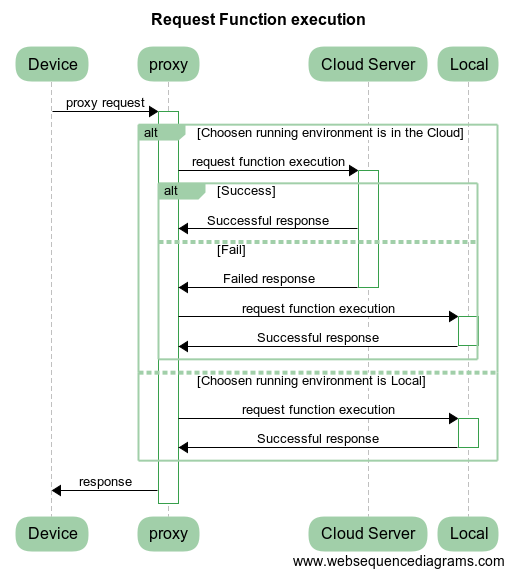
\includegraphics[width=0.5\textwidth]{diss-high-level-sequence-diagram.png}
    %\caption{High level sequence the whole process. This diagram sums the
        %decision-making of the project when trying to answer the request for the
        %function execution}
        %\label{fig:high_level_request_func_seq_diagram}
  %\end{center}
%\end{figure}


\section{Experimentation and evaluation}

\section{Conclusion}
The conclusion goes here.




% conference papers do not normally have an appendix


% use section* for acknowledgment
\section*{Acknowledgment}


The authors would like to thank...





% trigger a \newpage just before the given reference
% number - used to balance the columns on the last page
% adjust value as needed - may need to be readjusted if
% the document is modified later
%\IEEEtriggeratref{8}
% The "triggered" command can be changed if desired:
%\IEEEtriggercmd{\enlargethispage{-5in}}

% references section

% can use a bibliography generated by BibTeX as a .bbl file
% BibTeX documentation can be easily obtained at:
% http://www.ctan.org/tex-archive/biblio/bibtex/contrib/doc/
% The IEEEtran BibTeX style support page is at:
% http://www.michaelshell.org/tex/ieeetran/bibtex/
%\bibliographystyle{IEEEtran}
% argument is your BibTeX string definitions and bibliography database(s)
%\bibliography{IEEEabrv,../bib/paper}
%
% <OR> manually copy in the resultant .bbl file
% set second argument of \begin to the number of references
% (used to reserve space for the reference number labels box)
\begin{thebibliography}{1}

\bibitem{IEEEhowto:kopka}
H.~Kopka and P.~W. Daly, \emph{A Guide to \LaTeX}, 3rd~ed.\hskip 1em plus
  0.5em minus 0.4em\relax Harlow, England: Addison-Wesley, 1999.

\end{thebibliography}




% that's all folks
\end{document}
